%\section{A Wrinkle in Time}

\section{A New Semantics for \IML}

In this section, we introduce a new kind of model for interpreting formulas of $\IML$.
These new models, called \emph{weaved models}, are designed as a generalization of the hierarchical perspective on intuitionistic modal logic with the aim of making this model more explicit. Concretely, weaved models reflect the idea behind hierarchical models of interpreting formulas on a collection of related Kripke models organized in a meaningful way.
What makes weaved models particularly useful is that, they are compatible with important metatheoretic results, such as the finite model property. In this way, weaved models combine the conceptual clarity of hierarchical models with the formal strengths of birelational Kripke models.

\subsection{Weaved models}

We begin with a technical preliminary definition.

\begin{definition}\label[definition]{def:simulation}
        A \defn{simulation} from a Kripke model $\kmodel_1$ to a Kripke model $\kmodel_2$ is a non-empty binary relation $\Sim \subseteq (\Wkm[1] \times \Wkm[2])$ such that, for all $s_1 \in \Wkm[1]$ and $s_2 \in \Wkm[2]$, if $s_1 \Sim s_2$, then:
        \begin{description}
                \setlength{\itemsep}{0pt}
                \item[\textnormal{(add)}] if $p \in \Vkm[1](s_1)$, then, $p \in \Vkm[2](s_2)$;
                \item[\textnormal{(see)}] for all $s_3 \in \Wkm[1]$, if $s_1 \Rkm[1] s_3$, then, there is $s_4 \in \Wkm[2]$ such that $s_2 \Rkm[2] s_4$ and $s_3 \Sim s_4$.
        \end{description}
        The relation $\Sim$ is a \defn{seesaw simulation} from $\kmodel_1$ to $\kmodel_2$,
        denoted as $\Sim\colon\kmodel_1\fsim\kmodel_2$, if it is both: a simulation from $\kmodel_1$ to    $\kmodel_2$, and a simulation from $\ikmodel_1$ to    $\ikmodel_2$.
        Here, $\ikmodel_{i} = \tuple{\Qkm[i],\iRkm[i],\Vkm[i]}$ is the \defn{inverse} of $\kmodel[i]$ for $i \in \set{1,2}$.
\end{definition}

\begin{proposition}
        The following two conditions are equivalent:
        \begin{enumerate}[leftmargin=\parindent]
                \item $\Sim$ is a seesaw simulation from $\kmodel_1$ to $\kmodel_2$.
                \item $\Sim$ is a simulation such that: (saw) for all $s_3 \in \Wkm[1]$, if $s_3 \Rkm[1] s_1$, then, exists $s_4 \in \Wkm[2]$ such that $s_4 \Rkm[2] s_2$ and $s_3 \Sim s_4$.
        \end{enumerate}
        \lutz{is there some $s_1\Sim s_2$ missing in (2)?}
\end{proposition}

\begin{definition}\label[definition]{def:simulation}
	A \defn{forward and backwards simulation} (from now on, a simulation for simplicity) from a Kripke model $\kmodel_1$ to a Kripke model $\kmodel_2$ (notation: $\Sim\colon\kmodel_1\fsim\kmodel_2$) is a non-empty binary relation $\Sim \subseteq (\Wkm[1] \times \Wkm[2])$ such that, for all $s_1 \in \Wkm[1]$ and $s_2 \in \Wkm[2]$, if $s_1 \Sim s_2$, then:
	\begin{description}
		\setlength{\itemsep}{0pt}
		\item[\textnormal{(add)}] if $p \in \Vkm[1](s_1)$, then, $p \in \Vkm[2](s_2)$;
		\item[\textnormal{(forth)}] for all $s_3 \in \Wkm[1]$, if $s_1 \Rkm[1] s_3$, then, there is $s_4 \in \Wkm[2]$ such that $s_2 \Rkm[2] s_4$ and $s_3 \Sim s_4$;
		\item[\textnormal{(back)}] for all $s_3 \in \Wkm[1]$, if $s_3 \Rkm[1] s_1$, then, there is $s_4 \in \Wkm[2]$ such that $s_4 \Rkm[2] s_2$ and $s_3 \Sim s_4$.
	\end{description}
\lutz{what is this def doing here? isn't this the same as 3.1?}
\end{definition}

\begin{proposition}
        For every Kripke model $\kmodel$, the identity (or diagonal) relation $\Delta_{\Qkm}=\setof{(q,q)}{q\in\Qkm}$ is a seesaw simulation $\id_{\kmodel}\colon\kmodel \fsim \kmodel$. Moreover, the composition $\Sim\relcomp\Tim\colon \kmodel_1 \fsim \kmodel_3$ of seesaw simulations $\Sim\colon\kmodel_1 \fsim \kmodel_2$ and ${\Tim\colon\kmodel_2 \fsim \kmodel_3}$ is a seesaw simulation.
\end{proposition}

\todo{decide if we need to define inverse and composition of relations in the beginning}

We have adopted simulations as the foundational relational tool for connecting individual Kripke models. In fact, seesaw simulations turn out to be the right kind of simulation for organizing these models into the layered architecture characteristic of weaved models. Intuitively, the conditions (see) and (saw) that characterize a seesaw simulation correspond closely to conditions (b) and (c) in the definition of bi-relational models. The formal definition of weaved models will make clear how seesaw simulations are used to assemble individual Kripke models into a cohesive whole, while preserving a hierarchical organization. This definition also makes immediate how weaved models reflects the same underlying intuition as hierarchical models, but achieves it in a more flexible way.

\begin{definition}\label[definition]{def:wmodel:simulation}
    A \defn{weaved model} is a pair $\wmodel = \tuple{\Kwm, \Swm}$ where:
    \begin{enumerate}[leftmargin=\parindent]
        \setlength{\itemsep}{0pt}
        \item $\Kwm$ is a non-empty set of Kripke models;
        % \item $\Fbm$ is a preorder on $\kmodels$;
        \item $\Swm$ is a set of seesaw simulations on $\Kwm$ closed under identities and composition.
    \end{enumerate}
%%    We use $\kmodels_{\wmodel}$, and $\G_{\wmodel}$, to indicate $\kmodels$, and $\G$, respectively.
    For any weaved model $\wmodel$, we define the set
    \begin{equation}
        \Qwm=\setof{\pair{\kmodel}q}{\kmodel\in\Kwm\mbox{ and } q\in\Qkm}
    \end{equation}
    and on this set we define the binary relation
    \begin{equation}
        \Fwm=\setof{(\pair\kmodel q,\pair{\kmodel'}{q'})}{\mbox{there is ${\Sim\colon\kmodel\fsim\kmodel'} \in \Swm$ with $q\Sim q'$}}.
    \end{equation}
\end{definition}

\begin{proposition}\label[proposition]{prop:preorder:wmodel}
    Let $\wmodel$ be a weaved model. \!Then, $\Fwm$ is a preorder~on~$\Qwm$.
\end{proposition}

\Cref{prop:preorder:wmodel} shows that, although weaved models do not specify a future relation explicitly, such a relation can still be recovered from their internal organization via seesaw simulations. This stands in contrast to bi-relational and hierarchical models, where the future relation is built directly into their definition. This result highlights a key feature of weaved models: they preserve the essential idea of a hierarchical arrangement of Kripke models, but achieve this using simulations instead of rigid relational constraints of hierarchical models. This approach allows for greater flexibility while still supporting the logical properties we expect in an intuitionistic modal setting.

\begin{definition}\label[definition]{def:sat:wmodel:simulation}
    Let $\wmodel$ be a weaved model, and ${\pair \kmodel s} \in \Qwm$.
    Moreover, let $A$ be a formula.
    The \defn{forcing relation} $\wforces {\pair \kmodel s} A$ is defined inductively as:
%%    The relation $\wforces {\pair \kmodel s} A$ is defined recursively as:
    \[\begin{array}{lcl}
        \wforces {\pair \kmodel s} \bot
            & \text{iff} & \text{false} \\
        \wforces {\pair \kmodel s} p
            & \text{iff} & p \in \Vkm(s) \\
        \wforces {\pair \kmodel s} {B \land C}
            & \text{iff} & \wforces {\pair \kmodel s} B \text{ and } \wforces {\pair \kmodel s} C \\
        \wforces {\pair \kmodel s} {B \lor C}
            & \text{iff} & \wforces {\pair \kmodel s} B \text{ or } \wforces {\pair \kmodel s} C \\
        \wforces {\pair \kmodel s} {B \to C}
            & \text{iff} & \text{for all } {\pair {\kmodel'} t} \in \Qwm, \\
            && \quad \text{if } {\pair \kmodel s} \Fwm {\pair {\kmodel'} t} \text{, then, } \\
            && \qquad \text{if } \wforces {\pair {\kmodel'} t} B \text{, then, } \wforces {\pair {\kmodel'} t} C \\
        \wforces {\pair \kmodel s} \Diamond B & \text{iff}
            & \text{exists } t \in \Wkm \text{ such that } s \Rkm t \text{ and } \wforces {\pair \kmodel t} B \\
        \wforces {\pair \kmodel s} \Box B & \text{iff}
            & \text{for all } {\pair {\kmodel'} t} \in \Qwm, \\
            && \quad \text{if } {\pair \kmodel s} \Fwm {\pair {\kmodel'} t} \text{, then, } \\
            && \qquad \text{for all } u \in \Wof{\kmodel'}, \text{ if } t \Rof{\kmodel'} u \text{, then, } \wforces {\pair {\kmodel'} u} B.
    \end{array}\]
    We use $\nwforces {\pair \kmodel s} A$ to indicate the negation of $\wforces {\pair \kmodel s} A$.
    Immediately, $\nwforces {\pair \kmodel s} \bot$, and $\wforces {\pair \kmodel s} \lnot B$ iff for all $\kmodel' \in \Khm$, if $\kmodel \Fwm \kmodel'$, then, $\nwforces {\pair {\kmodel'} s} B$.
\end{definition}

With the forcing relation for weaved models in place, we turn our attention to commenting on some of its features as a semantic framework for intuitionistic modal logic.
The most basic of these features is monotonicity, made precise in \Cref{prop:monotonicity:ws} below.

\begin{proposition}[Monotonicity]\label[proposition]{prop:monotonicity:ws}
    Let $\wmodel$ be a weaved model, and $A$ be a formula.
    For all ${\pair {\kmodel_1} s}, {\pair {\kmodel_2} t} \in \Qwm$, if $\wforces{\pair {\kmodel_1} s}{A}$ and ${\pair {\kmodel_1} s} \Fwm {\pair {\kmodel_2} t}$, then, $\wforces {\pair {\kmodel_2} t} A$.
\end{proposition}
\begin{proof}
    %Suppose $\wforces{\pair \kmodel s}{A}$ and ${\pair \kmodel s} \Fwm {\pair {\kmodel'} t}$.
    We prove the result by a case analysis and induction on~$A$.

    \medskip
    \noindent
    For formulas of the form $p$, $B \to C$, and $\Box B$, the result follows from the fact that monotonicity is built into the definition of the forcing relation for weaved models.
    We illustrate the case of $\Box B$ as representative of this fact.
    Suppose that (1) $\wforces {\pair {\kmodel_1} s} \Box B$, and ${\pair {\kmodel_1} s} \Fwm {\pair {\kmodel_2} t}$ for an arbitrary ${{\pair {\kmodel_2} t} \in \Qwm}$.
    We need to establish $\wforces {\pair {\kmodel_2} t} \Box B$.
    We proceed by contradiction.
    Let ${\nwforces {\pair {\kmodel_2} t} \Box B}$.
    There are ${\pair {\kmodel_3} u} \in \Qwm$ and $v \in \Wkm[3]$ s.t.\ ${\pair {\kmodel_2} t} \Fwm {\pair {\kmodel_3} u}$, $u \Rkm[3] v$, and $\nwforces {\pair {\kmodel_3} v} B$.
    From the transitivity of $\Fwm$, ${\pair {\kmodel_1} s} \Fwm {\pair {\kmodel_3} u}$.
    But this fact contradicts (1).
    Therefore, $\wforces {\pair {\kmodel_2} t} \Box B$.

    \medskip
    \noindent
    The cases of conjunctions $B \land C$, disjunctions $B \lor C$, and diamonds $\Diamond B$ are proven by induction.
    The base cases are immediate.
    The inductive hypothesis assumes monotonicity holds for an arbitrary formula.
    We illustrate the case of $\Diamond B$ as representative of the reasoning involved in the inductive step.
    Suppose (2) ${\wforces {\pair {\kmodel_1} s} \Diamond B}$, and (3) ${\pair {\kmodel_1} s} \Fwm {\pair {\kmodel_2} t}$ for an arbitrary ${\pair {\kmodel_2} t} \in \Qwm$.
    We need to establish $\wforces {\pair {\kmodel_2} t} \Diamond B$.
    From (2), we know there is $u \in \Qkm[1]$ such that $s \Rkm[1] u$ and $\wforces {\pair {\kmodel_1} u} B$.
    From (3), we know there is a seesaw simulation $\Sim \colon {\kmodel_1 \fsim \kmodel_2} \in \Swm$ such that $s \Sim u$.
    The (see) condition ensures there is $v \in \Wkm[2]$ such that (4) $t \Rkm[2] v$ and $u \Sim v$. This guarantees that ${\pair{\kmodel_1}{u}} \Fwm {\pair{\kmodel_2}{v}}$. By the inductive hypothesis, we have $\wforces{\pair{\kmodel_2}{v}} B$. Combining this last step with (4), we conclude that $\wforces{\pair{\kmodel_2}{t}} \Diamond B$.
\end{proof}

The use of the (see) condition in the proof of \Cref{prop:monotonicity:ws} highlights its essential role in the definition of seesaw.
Intuitively, the condition serves the same purpose in weaved models as condition (b) in \Cref{def:bmodel} does for bi-relational models, and condition (b) in \Cref{def:imodel} does for hierarchical models. In each case, these conditions ensure that the modal accessibility relation behaves in a way that preserves the constructive, monotonic nature of the logic across related worlds.
The following example illustrates the role played by (saw) in the definition of a seesaw simulation.

\begin{example}\label[example]{ex:plotkin}
    \def\pwmodel{\mathfrak{S}}
    The model in \Cref{fig:weaved:plotkin} illustrates what can go wrong if we restrict ourselves to simulations instead of seesaw simulations in a weaved model.
    Formally, this model is the pair $\pwmodel = \tuple{\set{\kmodel_1, \kmodel_2}, \set{\id_{\kmodel_1}, \id_{\kmodel_2}, \Sim}}$, where:
        \[
            \kmodel_1 = \tuple{\set{s, t}, \set{(s, t)}, \Vkm[1]}
            \quad \text{and} \quad
            \kmodel_2 = \tuple{\set{u,v,w}, \set{(u, v)}, \Vkm[2]}
        \]
    are Kripke models with valuations $\Vkm[1](s) = \Vkm[1](t) = \Vkm[2](u) = \Vkm[2](v) = \emptyset$ and $\Vkm[2](w) = \set{p}$.
    The relation $\Sim = \set{(s, u), (t, v)}$ is a (total) simulation from $\kmodel_1$ to $\kmodel_2$ that is not a seesaw simulation.
    If we keep the semantic clauses from \Cref{def:sat:wmodel:simulation}, it is easy to verify that $\xforces{\pwmodel}{\pair{\kmodel_1}{s}}{\lnot \Diamond p}$ holds, while $\xforces{\pwmodel}{\pair{\kmodel_1}{s}}{\Box \lnot p}$ fails. Consequently, we obtain $\nxforces{\pwmodel}{\pair{\kmodel_1}{s}}{\lnot \Diamond p \to \Box \lnot p}$.
    This outcome conflicts with the intuition that the formula $\lnot \Diamond A \to \Box \lnot A$ should hold in an intuitionistic modal setting. Seesaw simulations---particularly the (saw) property---rule out exactly these kinds of counterexamples.
\end{example}

\begin{figure}[!t]
    \centering
    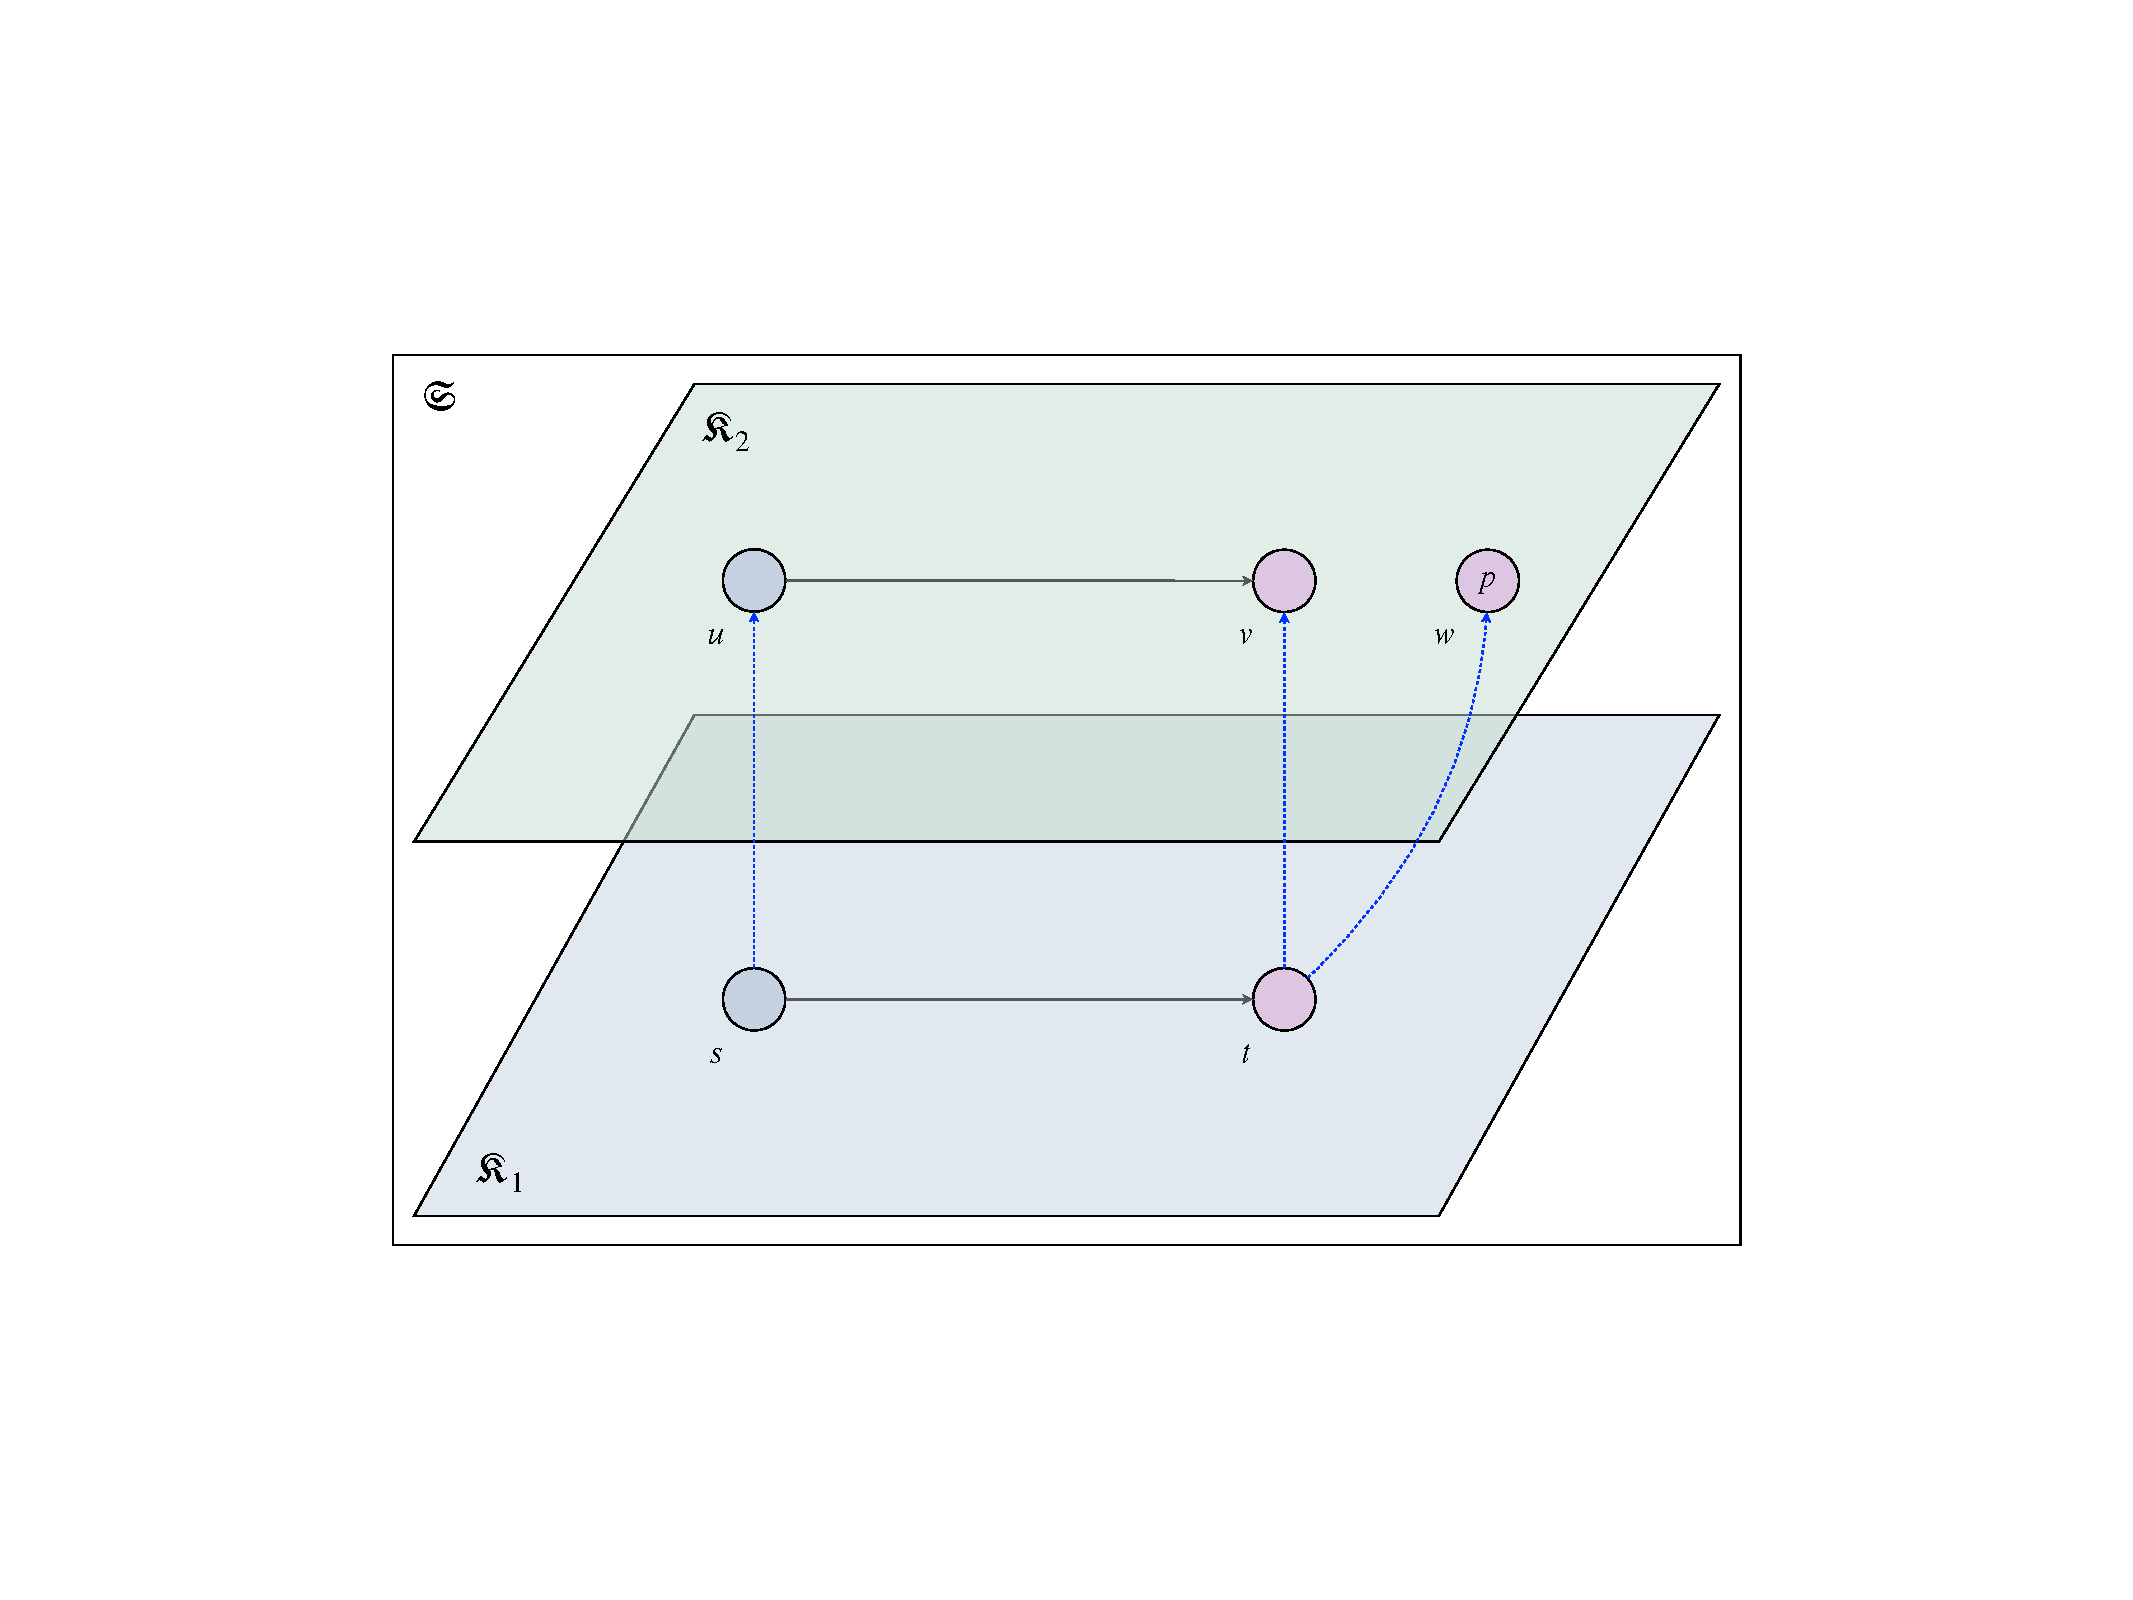
\includegraphics[height=4.9cm]{figures/plotkin.pdf}
    \caption{The Importance of (saw) in Seesaw Simulations}
    \label{fig:weaved:plotkin}
\end{figure}

The next result further elaborates on the point made in \Cref{ex:plotkin}.

\begin{proposition}
    Let $\wmodel$ be a weaved model.
    Then, for all ${\pair {\kmodel_1} s} \in \Qwm$, $\wforces{\pair {\kmodel_1} s}{\lnot \Diamond A \to \Box \lnot A}$.
\end{proposition}
\begin{proof}
    The proof is by contradiction.
    Let $\nwforces{\pair {\kmodel_1} s}{\lnot \Diamond A \to \Box \lnot A}$.
    There is ${\pair {\kmodel_2} t} \in \Qwm$ such that:
        (1) ${\pair {\kmodel_1} s} \Fwm {\pair {\kmodel_2} t}$,
        (2) $\wforces{\pair {\kmodel_2} t}{\lnot \Diamond A}$, and
        (3) $\nwforces{\pair {\kmodel_2} t}{\Box \lnot A}$.
    % From (2),
    %     for all ${\pair {\kmodel_3} u} \in \Qwm$,
    %         if ${\pair {\kmodel_2} t} \Fwm {\pair {\kmodel_3} u}$, then,
    %             $\nwforces{\pair {\kmodel_3} u}{\Diamond A}$.
    From (3),
        there are ${\pair {\kmodel_3} u} \in \Qwm$ and ${v \in \Wkm[3]}$ such that
            ${\pair {\kmodel_2} t} \Fwm {\pair {\kmodel_3} u}$,
            $u \Rkm[3] v$, and
            $\nwforces{\pair {\kmodel_3} v}{\lnot A}$.
    This implies there is ${\pair {\kmodel_4} w} \in \Qwm$ such that
        (4) ${\pair {\kmodel_3} v} \Fwm {\pair {\kmodel_4} w}$, and
        $\wforces{\pair {\kmodel_4} w}{A}$.
    From (4), there is $\Sim \colon \kmodel_3 \fsim \kmodel_4$ such that $v \Sim w$.
    By the (saw) property, there is $w \in \Wkm[4]$ such that $v \Sim x$ and $x \Rkm[4] w$.
    And so, $\wforces{\pair {\kmodel_4} x}{\Diamond A}$.
    But this fact contradicts (2), as we have
        ${\pair {\kmodel_2} t} \Fwm {\pair {\kmodel_4} x}$, and
        $\wforces{\pair {\kmodel_4} x}{\Diamond A}$.
\end{proof}

We are now in a position to reflect on weaved models from a more conceptual standpoint. To guide this discussion, we follow the perspective outlined in \cite{simpson1994}, where it is noted that, within the Kripkean framework for intuitionistic logic, atomic facts are expected to persist into the future. That is, if an atomic proposition holds at a given world, it must continue to hold at all future worlds.

This principle can be extended beyond propositional atoms to the accessibility relation itself. In particular, if we treat the statement \emph{a world sees another world} as a kind of structural atomic fact, then the accessibility relation becomes subject to the same persistence requirement. This view provides a conceptual foundation for condition (b) in \Cref{def:bmodel} for bi-relational models, condition (b) in \Cref{def:imodel} for hierarchical models, and the (see) condition in seesaw simulations for weaved models.
The dual perspective, i.e., treating \emph{a world is seen by another} also as a kind of structural atomic fact, supports condition (c) in both \Cref{def:bmodel} and \Cref{def:imodel}, and the (saw) property for seesaw simulations.

In a hierarchical or layered setting, the idea of persistence can be extended even further. If a world $w$ exists at one point in the hierarchy, then it is natural to expect that $w$ continues to exist in the future, possibly with additional information. This intuition is captured explicitly as condition (a) in \Cref{def:imodel}.
For weaved models, the situation is more nuanced. The persistence of worlds is not built into the model itself but is instead governed by the properties of the seesaw simulations. Totality of the simulation relation would ensure the persistence of all worlds, but since totality plays no essential technical role in our results, we have chosen to set it aside. In this respect, the kind of persistence of worlds needed in weaved models is supported by the combination of (see) and (saw).
That said, while (see) and (saw) collectively achieve the required semantic effects, we acknowledge that they lack the broader conceptual justification that totality enjoys within the Kripkean paradigm.

\lutz{this discussion might be great for a philopsophy journal, but it will kill the paper for LICS.}

\subsection{From Weaved to Bi-relational and hierarchical models (and Back)}

To better understand the role of weaved models within intuitionistic modal logic, we examine how they relate to bi-relational and hierarchical models. Precisely, we show how weaved models can be seen as a generalization encompassing both frameworks. This comparison not only clarifies the conceptual foundations of weaved models but also highlights their flexibility in capturing layered modal behavior.

% Let $\hmodel$ be a hierarchical model and $\kmodel_1,\kmodel_2\in\Khm$ with $\kmodel_1\Fhm\kmodel_2$. We define the relation $\Sof{\kmodel_1,\kmodel_2}=\Delta_{\Qkm[1]}\subseteq\Qkm[1]\times\Qkm[1]\subseteq\Qkm[1]\times\Qkm[2]$. By Proposition..... this is a seesaw simulation $\Sof{\kmodel_1,\kmodel_2}\colon\kmodel_1\fsim\kmodel_2$.

\begin{proposition}\label{prop:hs2ws}
    Let $\hmodel$ be a hierarchical model.
    % Define the pair $\wmofhm=\tuple{\Kof{\wmofhm},\Sof{\wmofhm}}$ where $\Kof{\wmofhm}=\Khm$ and $\Sof{\wmofhm}=\setof{\Sof{\kmodel_1,\kmodel_2}}{\kmodel_1\Fhm\kmodel_2}$.
    Then, the pair
        \[
            \wmofhm = \tuple{\Khm,\setof{\Wkm[1] \isym \Wkm[2]}{\kmodel_1 \Hleq \kmodel_2}}
            \footnote{For $X \subseteq Y$, $X \isym Y$ indicates the inclusion map, i.e., the mapping of $x \in X$ to $x \in Y$. \lutz{don't make this a footnote. that should be in the main text}}
        \] 
    satisfies the following properties:
    %% It follows that:
    \begin{enumerate}[leftmargin=\parindent]
        \setlength{\itemsep}{0pt}
        \item $\wmofhm$ is a weaved model.
        \item $\hmodel$ is finite implies $\wmofhm$ is finite.
        \item $\hforces{\pair\kmodel s}A$ ~iff~ $\xforces{\wmofhm}{\pair\kmodel s} A$.
    \end{enumerate}
\end{proposition}
\begin{proof}
    Let $\wmofhm = \tuple{\Khm, \Swm}$.
    For item (1), it suffices to show that all inclusion maps ${\Wkm[1] \isym \Wkm[2]} \in \Swm$ are seesaw simulations, and that $\Swm$ is closed by identities and composition. But this follows immediately from the definition.
    Item (2) is similarly straightforward.
    For item (3), note that the forcing relation for weaved models aligns with that of hierarchical models, if all seesaw simulations are total and functional relations. If in addition the seesaw relations are inclusion maps, the semantics behaves identically across both settings.
\end{proof}

In brief, \Cref{prop:hs2bks} reveals that hierarchical models can be viewed as a special case of weaved models---those in which the connecting seesaw simulations are inclusion maps. Conceptually, this further highlights how weaved models capture the same foundational idea of layering Kripke models over time, but with greater flexibility: instead of requiring rigid inclusions, they allow more general relational connections while preserving the essential intuitionistic modal behavior.

\begin{proposition}\label[proposition]{prop:ws2bks}
    %% Let $\wmodel$ be a weaved model.
    %% Also, let $\bmodel_{\wmodel} = \tuple{\W, {\preccurlyeq}, \R, \V}$ be s.t.:
    %% \begin{enumerate}[leftmargin=\parindent]
    %%     \setlength{\itemsep}{0pt}
    %%     \item $\W = \setof{(\kmodel, s)}{ \kmodel \in \kmodels_{\wmodel} \text{ and } s \in \W_{\kmodel}}$;
    %%     \item ${\preccurlyeq} = \setof{ (\bb{s}, \bb{t}) }{ {f:{\bb{s}_1 \to \bb{t}_1} \in \Swm} \text{ and } {f(\bb{s}_2) = \bb{t}_2}}$;
    %%     \item $\R = \setof{ (\bb{s}, \bb{t}) }{ \set{\bb{s}_1, \bb{t}_1} \subseteq \kmodels_{\wmodel} \text{ and } {\bb{s}_1 = \bb{t}_1} \text{ and } {\bb{s}_2 \R_{\bb{s}_1} \bb{t}_2}}$;
    %%     \item %$\V_{\wmodel}: \props \to 2^{\S_{\wmodel}}$ is s.t.\
    %%         for all $\bb{s} \in \W$, $\V(s) = \V_{\bb{s}_1}(\bb{s}_2)$.
    %% \end{enumerate}
    %% It follows that:
    %% \begin{enumerate}[label=(\alph*)]
    %%     \setlength{\itemsep}{0pt}
    %%     \item $\bmodel_{\wmodel}$ is a bi-relational Kripke model; and
    %%     \item $\wforces {\pair \kmodel s} A$ iff $\xforces {\bmofwm} {\pair{\kmodel}{s}} \Vdash A$.
    %%     \item $\wmodel$ is finite implies $\bmodel_{\wmodel}$ is finite;
    %% \end{enumerate}
    Let $\wmodel$ be a weaved model.
    Define the quadruple
        \[
            \bmofwm = \tuple{\Qwm, \Fwm, \R, \V}
        \]
    where:
    \begin{enumerate}[leftmargin=\parindent,label=(\roman*)]
        \setlength{\itemsep}{0pt}
        % \item $\Wof{\bmofwm} = \setof{\pair\kmodel s}{ \kmodel \in \kmodels_{\wmodel} \text{ and } s \in \W_{\kmodel}}$;
        % \item $\Fof{\bmofwm} = \setof{ (\pair{\kmodel_1}{q_1}, \pair{\kmodel_2}{q_2}) }{\text{there is a }\Sim\colon \kmodel_1 \fsim\kmodel_2 \text{ in }\Swm \text{ and } q_1\Sim q_2}$;
        \item $\R    = \setof{ (\pair{\kmodel}{s_1}, \pair{\kmodel}{s_2}) }{ \kmodel\in \Kwm \text{ and } s_1 \Rkm s_2}$;
        \item %$\V_{\hmodel}: \props \to 2^{\S_{\hmodel}}$ is s.t.\
            for all $\pair\kmodel s \in \Qwm$, $\V(\npair \kmodel s) = \Vkm(s)$.
    \end{enumerate}
    It follows that:
    \begin{enumerate}[leftmargin=\parindent]
        \setlength{\itemsep}{0pt}
        \item $\bmofwm$ is a    birelational model; and
        \item if $\wmodel$ is finite then    $\bmofwm$ is finite;
        \item $\wforces{\pair\kmodel s} A$ ~iff~ $\xforces{\bmofwm}{\pair\kmodel s} A$.
    \end{enumerate}
\end{proposition}
\begin{proof}
    For item (1), we have proven in \Cref{prop:preorder:wmodel} that $\Fwm$ is a preorder on $\Qwm$.
    We still need to prove that it satisfies conditions (a)--(c) in \Cref{def:bmodel}.
    For (a), suppose that $p \in \V(\npair {\kmodel_1} s)$ and ${\pair {\kmodel_1} s} \Fwm {\pair {\kmodel_2} t}$.
    From the definition of $\V$, we have $p \in \Vkm[1](s)$.
    From the definition of $\Fwm$, there is a seesaw simulation $\Sim \in \Swm$ such that $s \Sim t$.
    Condition (add) in the definition of a simulation guarantees $p \in \Vkm[2](t)$.
    This fact establishes $\V(\npair {\kmodel_2} t)$ as required.
    For (b), suppose that ${\pair {\kmodel_1} s} \Fwm {\pair {\kmodel_2} t}$ and ${\pair {\kmodel_1} s} \R {\pair {\kmodel_3} u}$.
    Again, from the definition of $\Fwm$, there is a seesaw simulation $\Sim \in \Swm$ such that $s \Sim t$.
    Moreover, from the definition of $\R$, we know $\kmodel_1 = \kmodel_3$ and $s \Rkm[1] u$.
    The (see) condition in a simulation guarantees there is $v \in \Wkm[2]$ such that $u \Sim v$ and $t \Rkm[2] v$.
    These two facts together give us ${\pair {\kmodel_3} u} \Fwm {\pair {\kmodel_2} v}$ and ${\pair {\kmodel_2} t} \R {\pair {\kmodel_2} v}$ as required.
    Finally, condition (c), follows similarly using the (saw) property of seesaw simulations.

    \medskip
    \noindent
    For item (3), the proof is by induction on $A$.

    \medskip
    \noindent
    The base case is: $\wforces {\pair \kmodel s} p$ iff $\xforces {\bmofwm} {\pair{\kmodel}{s}} p$.
    This result follows directly from the fact that $\V(\npair \kmodel s) = \Vkm(s)$.
    
    \medskip
    \noindent
    The inductive step proceeds with a case analysis.
    We prove the cases of $\Box B$ and $\Diamond B$ as representative of the kind of reasoning involved.

    \medskip
    \noindent
    For boxes, we must show $\wforces {\pair {\kmodel_1} s} \Box B$ iff $\xforces {\bmofwm} {\pair{\kmodel_1}{s}} \Box B$.
    From left-to-right, suppose (i) $\wforces {\pair {\kmodel_1} s} \Box B$.
    Choose arbitrary ${\pair {\kmodel_2} t}, {\pair {\kmodel_3} u} \in~\Qwm$ such that:
        (ii) ${\pair {\kmodel_1} s} \Fwm {\pair {\kmodel_2} t}$, and
        (iii) ${\pair {\kmodel_3} t} \R {\pair {\kmodel_3} u}$.
    From (i)--(iii), it follows that $\wforces {\pair {\kmodel_3} u} B$.
    By the inductive hypothesis, $\xforces {\bmofwm} {\pair {\kmodel_3} u} B$.
    This last step, together with (ii) and (iii), gives us $\xforces {\bmofwm} {\pair{\kmodel_1}{s}} \Box B$ as required.
    The right-to-left implication uses a similar argument.

    \medskip
    \noindent
    For diamonds, we must show $\wforces {\pair \kmodel s} \Diamond B$ iff $\xforces {\bmofwm} {\pair{\kmodel}{s}} \Diamond B$.
    From left-to-right, suppose $\wforces {\pair \kmodel s} \Diamond B$.
    Then, there is $t \in \Wkm$ such that $s \Rkm t$ and (iv) $\wforces {\pair \kmodel t} B$.
    By definition, there is ${\pair \kmodel t} \in \Qwm$ such that ${\pair \kmodel s} \R {\pair \kmodel t}$.
    Using the inductive hypothesis on (iv), we get $\xforces {\bmofwm} {\pair{\kmodel}{t}} B$.
    The last two steps together yield $\bmodel_{\wmodel}, (\kmodel, s) \Vdash \Diamond B$ as required.
    The right-to-left implication uses a similar argument.
\end{proof}

% \valentin{Revised up to here. To be continued ...}

The following proposition is obtained immediately

\begin{proposition}
    Let $\hmodel$ be a hierarchical model. Then, $\bmofhm = \bmodel(\wmofhm)$.
\end{proposition}

We now turn to the task of translating bi-relational models into weaved models. It turns out that this translation is not uniquely determined---there are multiple ways to carry it out. However, we will see that two particular translations stand out as \emph{canonical}.

\begin{construction}\label{con:bks2ws}
Let $\bmodel$ be a birelational model. A \defn{partition} of $\bmodel$ is a set $\QQs=\setof{\Qof i}{i\in\Ind}$ where $\Ind$ is some index set, such that
\begin{enumerate}
\item $\bigcup_{i\in\Ind}\Qof i = \Qbm$
\item for all $i,j\in\Ind$ with $i\neq j$ we have $\Qof i \cap \Qof j=\emptyset$ 
\item for all $i,j\in\Ind$ with $i\neq j$ we have
    $\Rbm\cap((\Qof i \times \Qof j)\cup(\Qof j \times \Qof i))=\emptyset$ 
\end{enumerate}
i.e, the sets in $\QQs$ are mutually disjoint and cover all of $\Qbm$,    and there is no $\Rbm$-edge connecting two different sets in $\QQs$. Now we can define for each $i\in\Ind$ a Kripke model by restricting $\kmofbm=\tuple{\Qbm,\Rbm,\Vbm}$ to $\Qof i$, i.e.,
$\kmodel[i]= \tuple{\Qof i, \Rof i, \Vof i}$ where $\Rof i=\Rbm\cap(\Qof i \times \Qof i)$ and $\Vof i= \restr{\Vbm}{\Qof i}$.
And for all $i,j\in \Ind$, we define $\Sof{i,j}=\Fbm\cap(\Qof i \times \Qof j)$.
    Now we can define $$\wmofbm\QQs = \tuple{\setof{\kmodel[i]}{i\in\Ind},\setof{\Sof {i,j}}{i,j\in\Ind \mbox{ and } \Sof {i,j}\neq\emptyset}}$$.
    \end{construction}

\valentin{I propose the following reformulation of construction~\ref{con:bks2ws}}

\lutz{I like the first one a bit better, but in fact, it should be a mix of the two. I'll make it later}
\begin{definition}\label[definition]{def:bks2ws}
    Let $\bmodel$ be a birelational model.
    A \defn{partition} of $\bmodel$ is a subset $\QQs \subseteq 2^{\Qbm}$ such that:
    \begin{enumerate}[leftmargin=\parindent]
        \setlength{\itemsep}{0pt}
        \item $\QQs$ is a partition of $\Qbm$; and
        \item for all $\Q,\Q' \in \QQs$, if $\Q \neq \Q'$, then
                $\Rbm\cap((\Q \times \Q')\cup(\Q' \times \Q))=\emptyset$.
    \end{enumerate}
    Moreover, for every for all $\Q,\Q' \in \QQs$, define:
    \begin{enumerate}[leftmargin=\parindent,resume]
        \setlength{\itemsep}{0pt}
        \item $\kmodel({\Q}) = \tuple{\Q, {\Rbm\cap(\Q \times \Q)}, \restr{\Vbm}{\Q}}$; and
        \item $\Sim(\npair \Q {\Q'}) = \Fbm\cap(\Q \times \Q')$.
    \end{enumerate}
    Finally, define $\wmofbm\QQs = \tuple{\Kof{}, \Sims}$ where:
    \begin{enumerate}[leftmargin=\parindent,resume]
        \setlength{\itemsep}{0pt}
        \item $\Kof{} = \setof{\kmodel(\Q)}{\Q \in \QQs}$;
        \item $\Sof{0} = \setof{\Sim(\npair {\Q} {\Q'})}{ \Q,\Q' \in \QQs \mbox{ and } {\Sim(\npair \Q {\Q'})}\neq\emptyset}$; and %\cup \setof{\Delta_{\Q}}{\Q \in \QQs}$.
        \item $\Sims$ is the closure of $\Sof{0}$ under identities and composition.
    \end{enumerate}
\end{definition}

Intuitively, a partition $\QQs$ of a bi-relational model $\bmodel$ breaks it into a collection of (relational) Kripke models $\kmodel(\Q)$, each corresponding to a block $\Q$ in the partition. Condition (2) in \Cref{def:bks2ws} ensures that each Kripke model is internally coherent: all accessibility relations must remain within a single slice. That is, if $\kmodel(\Q)$ and $\kmodel(\Q')$ are Kripke models built from distinct partition blocks, no accessibility relation can connect a world in $\Q$ to one in $\Q'$.
Condition (3) in \Cref{def:bks2ws}, specifies how different slices are related to one another, capturing a sense of progression across slices.
The model $\wmofbm\QQs$ then organizes these slices into a layered arrangement that reflects their interrelation. As we will show in the next result, this organization aligns precisely with the hierarchical architecture of weaved models.

\begin{proposition}\label[proposition]{prop:bks2ws}
    Let $\bmodel$ be a bi-relational Kripke model, and $\QQs$ be a partition of $\bmodel$.
    We have that:
    \begin{enumerate}[leftmargin=\parindent]
        \setlength{\itemsep}{0pt}
        \item $\wmofbm\QQs$ is a weaved model;
        \item if $\bmodel$ is finite then $\wmofbm\QQs$ is finite; and
        \item For all $\Q\in\QQs$ and $s\in \Q$, we have $\bforces s A$ ~iff~ $\xforces{\wmofbm\QQs} {\pair{\kmodel(\Q)} s} A$
    \end{enumerate}
\end{proposition}

\begin{proof}
    Let $\wmofbm{\QQs} = \tuple{\Kof{}, \Sims}$.
    For item (1), we need to prove that $\Sims$ is a set of seesaw simulations and that it is closed by identities and composition.
    Suppose $\Sim \in \Sims$ is a relation from $\Q$ to $\Q'$, with $\Q,\Q' \in \QQs$.
    We proceed to prove that $\Sim$ is a seesaw simulation, i.e., that it satisfies (add), (see), and (saw).
    Choose arbitrary $s \in \Q$ and $t \in \Q'$ with $s \Sim t$.
    From the definition of $\Sim$, we know $s \Fbm t$.
    From \Cref{def:bmodel}, $\Vbm(s) \subseteq \Vbm(t)$.
    This fact implies $\Sim$ satisfies (add).
    Moreover, suppose that there is $u \in \Q$ such that $s \Rof{\kmodel(\Q)} u$.
    Immediately, $s \Rbm u$.
    From condition (b) in \Cref{def:bmodel}, we know there is $v \in \Wbm$ such that (i) $t \Rbm v$ and (ii) $u \Fbm v$.
    From (i) and condition (2) in the definition of a partition, we know $t \Rof{\kmodel(\Q')} v$ and $v \in \Q'$.
    This last fact combined with (ii) implies $u \Sim v$.
    Therefore, $\Sim$ satisfies (see).
    A similar argument shows that $\Sim$ satisfies (saw).
    That $\Sims$ contains all identities and is closed under composition is immediate from its definition.
    This concludes the proof of item (1).

    \medskip
    \noindent
    For item (3), the proof is by induction on $A$.
    To simply the notation, we use $\wmodel$ instead of $\wmofbm\QQs$.
    We also assume $\Q \in \QQs$ and $s \in \Q$ are arbitrary.

    \medskip
    \noindent
    The base case is: $\bforces s p$ iff $\xforces {\wmodel} {\pair {\kmodel(\Q)} {s}} p$.
    This result is direct from the fact that $s \in \Q$, which yields $\Vbm(s) = \restr{\Vbm}{\Q}(s) =\Vof{\kmodel(\Q)}(s)$.
    
    \medskip
    \noindent
    The inductive step proceeds with a case analysis.
    We prove the cases of $\Box B$ and $\Diamond B$ as representative of the kind of reasoning involved.

    \medskip
    \noindent
    For boxes, we must show $\bforces s {\Box B}$ iff $\xforces {\wmodel} {\pair {\kmodel(\Q)} s} {\Box B}$.
    From left-to-right, suppose (i) $\bforces s \Box B$.
    Choose arbitrary ${\pair {\kmodel(\Q')} t} \in \Kof{\wmodel}$ and $u \in \Q'$ such that:
        (ii) ${\pair {\kmodel(\Q)} s} \Fof{\wmodel} {\pair {\kmodel(\Q')} t}$, and
        (iii) $t \Rof{\kmodel(\Q')} u$.
    From (ii) and (iii), it follows that $s \Fbm t$ and $t \Rbm u$.
    Thus, from (i), we have $\bforces s B$.
    By the inductive hypothesis, $\xforces {\wmodel} {\pair {\kmodel(\Q')} u} B$.
    This last fact, together with (ii) and (iii), gives us $\xforces {\wmodel} {\pair{\kmodel(\Q)}{s}} {\Box B}$ as required.
    The right-to-left implication uses a similar argument.

    \medskip
    \noindent
    For diamonds, we must show $\bforces s {\Diamond B}$ iff $\xforces {\wmodel} {\pair {\kmodel(\Q)} {s}} {\Diamond B}$.
    From left-to-right, suppose $\bforces s {\Diamond B}$.
    Then, there is $t \in \Wbm$ such that (iv) $s \Rbm t$ and (v) $\bforces t B$.
    From (iv) and condition (2) in \Cref{def:bks2ws}, we know there is (vi) $t \in \Q$ and $s \Rof{\kmodel(\Q)} t$.
    Using the inductive hypothesis on (v), we have $\xforces {\wmodel} {\pair {\kmodel(\Q)} t} B$.
    This last step, together with (vi), gives us $\xforces {\wmodel} {\pair {\kmodel(\Q)} s} {\Diamond B}$ as required.
    The right-to-left implication uses a similar argument.
\end{proof}

We point out that, although any partition of a bi-relational model gives rise to a weaved model, two partitions are especially noteworthy and can be considered ``canonical'' in a natural sense.
The first is the trivial partition, where all worlds are grouped into a single block: $\QQs[0] = {\Qbm}$. This leads to the weaved model $\wmofbm0 = \tuple{\set{\tuple{\Qbm, \Rbm, \Vbm}}, \set{\Fbm, \Delta_{\Qbm}}}$, where $\Fbm$ acts as a seesaw simulation on the entire set of worlds $\Qbm$.
The second canonical partition, denoted $\QQs[\ast]$, divides $\Qbm$ into blocks that correspond to the connected components of the graph $\tuple{\Qbm, \Rbm}$. That is, each block contains the set of worlds that are path-connected via $\Rbm$. We write $\wmofbm\ast$ for the weaved model generated from this partition.
In both cases, the resulting weaved models reveal the hierarchical organization of Kripke models implicitly encoded in the bi-relational framework.

\begin{figure*}[!t]
	\centering
	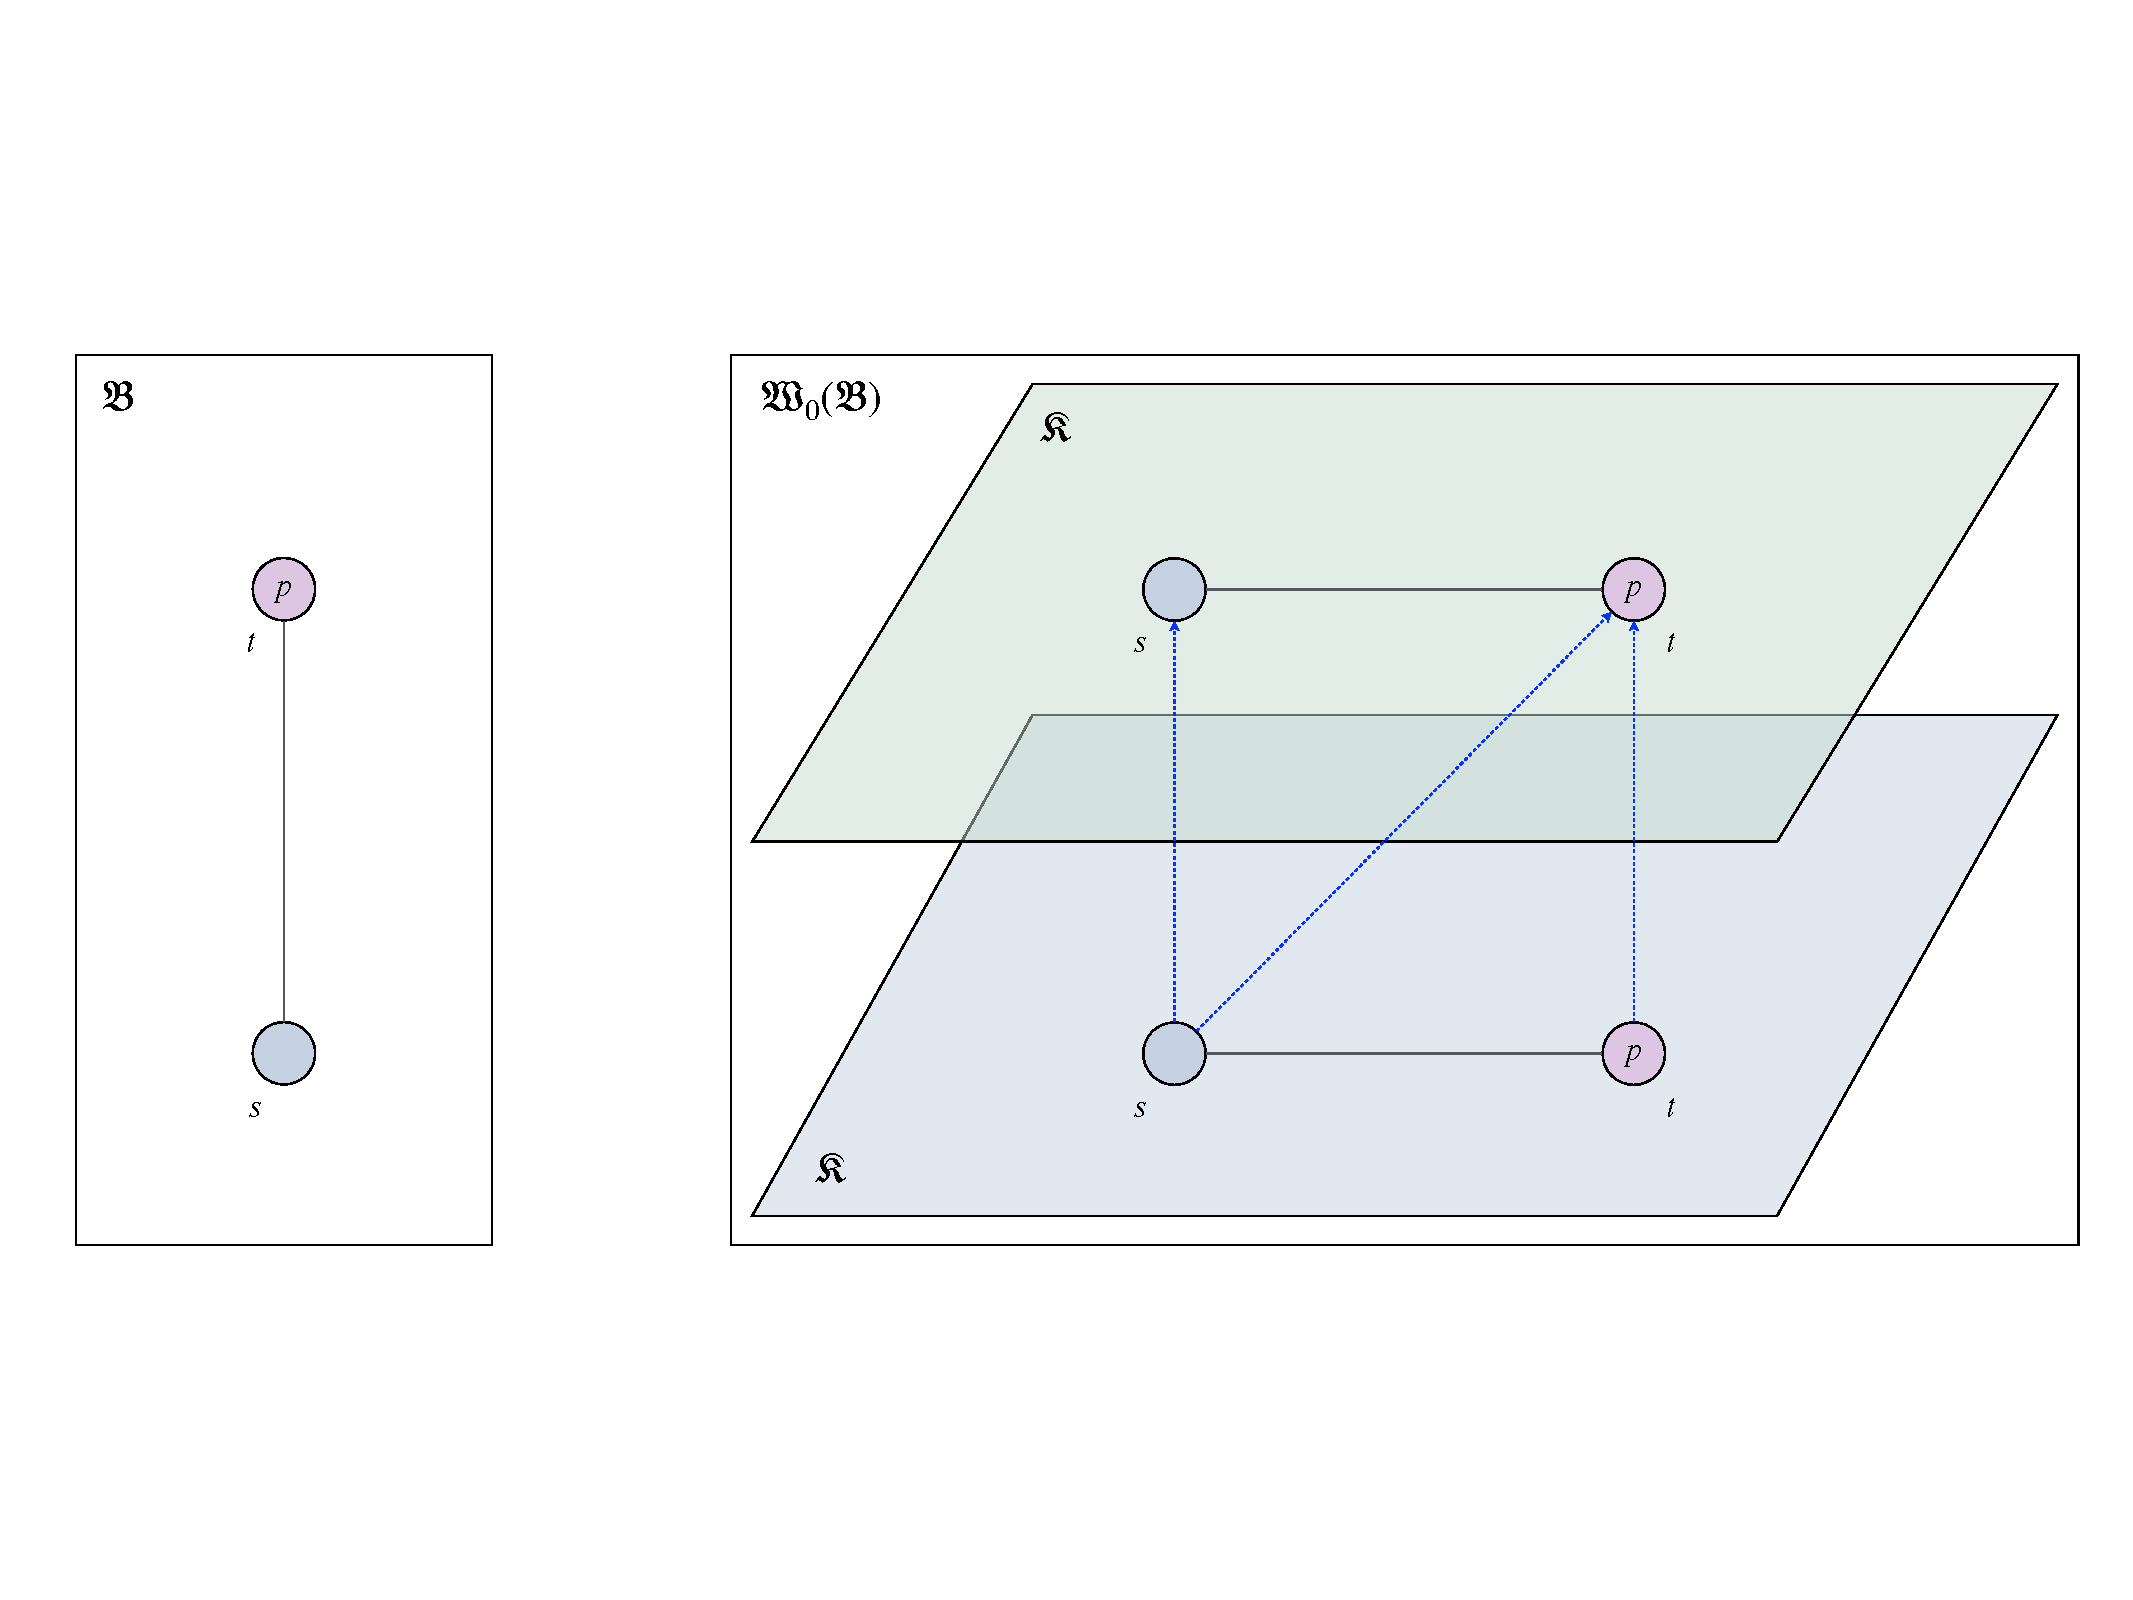
\includegraphics[height=4.9cm]{figures/bks2ws.pdf}
	\caption{Bi-relational Kripke model to Weaved model}
	\label{fig:bks2ws}
\end{figure*}

\begin{example}
        Let $\bmodel$ be the bi-relational model defined by $\Wbm = \set{s, t}$, with $\Fbm = \Delta_{\Wbm} \cup \set{\pair s t}$ and $\Rbm = \set{{\pair s t},{\pair t s}}$. The valuation function is given by $\Vbm(s) = \emptyset$ and $\Vbm(t) = {p}$. This model is depicted on the left side of \Cref{fig:bks2ws}. In the diagram, solid arrows represent the accessibility relation $\Rbm$, and the vertical placement of $t$ above $s$ visually encodes the future pair $s \Fbm t$.

        The weaved model $\wmofbm0$ obtained by applying the construction from \Cref{def:bks2ws} to $\bmodel$ using the trivial partition $\QQs = \set{\set{s, t}}$ is depicted on the right side of \Cref{fig:bks2ws}. In this depiction, the future relation $\Fbm$---now acting as a seesaw simulation from $\kmodel(\set{s, t})$ to itself---is represented by dotted blue arrows.
        To better highlight the hierarchical organization induced by $\Fbm$ within the single Kripke model $\kmodel(\set{s, t}) \in \Kof{\wmofbm0}$, we present it as if there were two stacked copies of the model, rather than illustrating the seesaw simulation as a loop. This visual choice emphasizes the layered nature typical of weaved models.

        \Cref{prop:bks2ws} allows us to compare the evaluation of formulas in $\bmodel$ and $\wmofbm0$.
        It is possible to verify that $\bforces s {\Box\lnot\lnot p}$ and $\nbforces s {\lnot\lnot\Box p}$; and so that $\xforces {\wmofbm0} {\pair {\set{s,t}} s} {\Box\lnot\lnot p}$ and $\nxforces {\wmofbm0} {\pair {\set{s,t}} s} {\lnot\lnot\Box p}$.
        We show the side-by-side evaluation of $\Box\lnot\lnot p$ in $\bmodel$ and $\wmofbm0$ in \Cref{fig:eval}.

        \begin{figure*}
                \begin{center}
                \resizebox{\textwidth}{!}{
                \fbox{
                \begin{minipage}[t]{.55\textwidth}
                        \begin{description}

                        \item[$\bforces s {\Box\lnot\lnot p}$]
                        \item[for all $\Fbm$] \hfil
                        \item[$s \Fbm s$] \hfil
                        \begin{description}
                                \item[for all $\Rbm$]
                                \item[$s \Rbm t$]\hfil
                                \begin{description}
                                \item[$\bforces t {\lnot\lnot p}$]
                                \item[for all $\Fbm$]
                                \item[$t \Fbm t$]\hfil
                                \begin{description}
                                        \item[$\nbforces t {\lnot p}$] \hfil
                                        \begin{description}
                                        \item[exists $\Fbm$]
                                        \item[$t \Fbm t$] \hfil
                                        \item[\quad] $\bforces t p$
                                        \end{description}
                                \end{description}
                                \end{description}
                        \end{description}

                        \item[$s \Fbm t$]\hfil
                        \begin{description}
                                \item[for all $\Rbm$]
                                \item[$t \Rbm s$]\hfil
                                \begin{description}
                                \item[$\bforces s {\lnot\lnot p}$]
                                \item[for all $\Fbm$]
                                
                                \item[$s \Fbm s$]\hfil
                                \begin{description}
                                        \item[$\nbforces s {\lnot p}$] \hfil
                                        \begin{description}
                                        \item[exists $\Fbm$]
                                        \item[$s \Fbm t$] \hfil
                                        \item[\quad] $\bforces t p$
                                        \end{description}
                                \end{description}
                                
                                \item[$s \Fbm t$]\hfil
                                \begin{description}
                                        \item[$\nbforces t {\lnot p}$] \hfil
                                        \begin{description}
                                        \item[exists $\Fbm$]
                                        \item[$t \Fbm t$] \hfil
                                        \item[\quad] $\bforces t p$
                                        \end{description}
                                \end{description}
                                \end{description}
                        \end{description}

                        \end{description}
                \end{minipage}}
                %
                \hfill
                %
                \fbox{
                \begin{minipage}[t]{.55\textwidth}
                        \begin{description}

                        \item[$\xforces {\wmofbm0} {\pair \kmodel s} {\Box\lnot\lnot p}$]
                        \item[for all $\Fof{\wmofbm0}$] \hfil
                        
                        \item[${\pair \kmodel s} \Fof{\wmofbm0} {\pair \kmodel s}$] \hfil
                        \begin{description}
                                \item[for all $\Rkm$]
                                \item[$s \Rkm t$] \hfil
                                \begin{description}
                                \item[$\xforces {\wmofbm0} {\pair \kmodel t} {\lnot\lnot p}$]
                                \item[for all $\Fof{\wmofbm0}$]
                                \item[${\pair \kmodel t} \Fof{\wmofbm0} {\pair \kmodel t}$]\hfil
                                \begin{description}
                                        \item[$\nxforces {\wmofbm0} {\pair \kmodel t} {\lnot p}$]
                                        \item[exists $\Fof{\wmofbm0}$]
                                        \item[${\pair \kmodel t} \Fof{\wmofbm0} {\pair \kmodel t}$]\hfil
                                        \item[\quad] $\xforces {\wmofbm0} {\pair \kmodel t} p$
                                \end{description}
                                \end{description}
                        \end{description}
                        
                        \item[${\pair \kmodel s} \Fof{\wmofbm0} {\pair \kmodel t}$] \hfil
                        \begin{description}
                                \item[for all $\Rkm$]
                                \item[$t \Rkm s$]\hfil
                                \begin{description}
                                \item[$\xforces {\wmodel} {\pair \kmodel s} \lnot\lnot p$]
                                \item[for all $\Fof{\wmofbm0}$]
                                
                                \item[${\pair \kmodel s} \Fof{\wmofbm0} {\pair \kmodel s}$]\hfil
                                \begin{description}
                                        \item[$\nxforces {\wmofbm0} {\pair \kmodel s} {\lnot p}$]
                                        \item[exists $\Fof{\wmofbm0}$]
                                        \item[${\pair \kmodel s} \Fof{\wmofbm0} {\pair \kmodel t}$]\hfil
                                        \item[\quad] $\xforces {\wmofbm0} {\pair \kmodel t} p$
                                \end{description}

                                \item[${\pair \kmodel s} \Fof{\wmofbm0} {\pair \kmodel t}$]\hfil
                                \begin{description}
                                        \item[$\nxforces {\wmofbm0} {\pair \kmodel t} {\lnot p}$]
                                        \item[exists $\Fof{\wmofbm0}$]
                                        \item[${\pair \kmodel t} \Fof{\wmofbm0} {\pair \kmodel t}$]\hfil
                                        \item[\quad] $\xforces {\wmofbm0} {\pair \kmodel t} p$
                                \end{description}
                                \end{description}
                        \end{description}
                        \end{description}
                \end{minipage}}
                }
                \end{center}
                \caption{Side-by-side Evaluation}\label{fig:eval}\lutz{this figure doesn't help at all with the understanding of the paper}
        \end{figure*}
\end{example}
